\section{Navigation}

As our website will be used by cell phones or computers, it is important to develop a design which supports user navigation, printing, etc. For this, we will use a single-screen design and navigation tools.

\subsection{General design}

Nowadays, there are a lot of tools which be able to access our website and each of them has probably different size of screen. It is better to use a single-screen design than a predefined size of screens (for example 800x600). It assures a good navigation whatever the tool. 

It is also important to establish a compromise between separate pages and scrolling long page. User doesn't like to scroll pages but if there are too many pages, he will be lost.


\subsection{Global systems}

On the top of all pages and just at the right of the website logo, which will be on the top left hand corner, will take place the global navigation systems. As defined in the section
%TODO ~\ref{} 
, the menu (figure \ref{fig:globalMenu}) is be composed of the followings groups: Boy, Girl, Clearance and Second Hand.

\begin{figure}[h!]
  \centering  
  
\includegraphics[width=0.5\textwidth]{Images/globalMenu.jpg}                
  \caption{Global navigation menu}
  \label{fig:globalMenu}
\end{figure}


\subsection{Local systems}
The local menu is on the left of all pages (except the home page) under the logo and the global menu. When you select, in a sidebar, one of the previous groups, you have access to the subgroups as defined in section
%TODO ~\ref{}
. For each subgroup (except Dresses, Bodysuits and Pajamas), you can also select a subsubgroup in the cascading menu. The figure \ref{fig:localMenu} shows examples for the Boy's local menu.

\begin{figure}[h!]
  \centering
  \subfloat[Sublocal menu for Tops]{\label{fig:localMenuTops}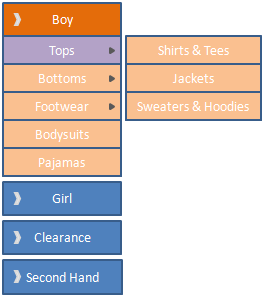
\includegraphics[width=0.35\textwidth]{Images/localMenuTops.png}}                
  \subfloat[Sublocal menu for Bottoms]
  {\label{fig:localMenuBottoms}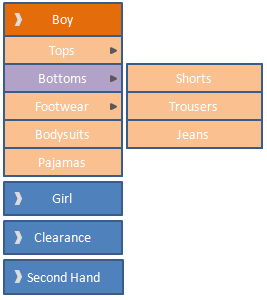
\includegraphics[width=0.35\textwidth]{Images/localMenuBottoms.png}}
  \subfloat[Sublocal menu for Footwear]{\label{fig:localMenuFootwear}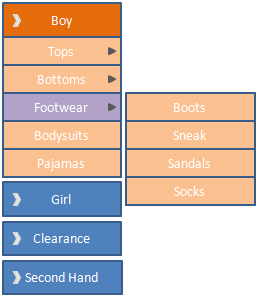
\includegraphics[width=0.35\textwidth]{Images/localMenuFootwear.png}}
  \caption{Local menu for Boys}
  \label{fig:localMenu}
\end{figure}

\subsection{Contextual and Supplemental systems}
In addition to using contextual navigation systems like hypertext links or associative links, ``also bought'' list and ``you may also like'' list, users can use supplemental navigation tools like Search bar and Breadcrumbs, which are very useful for finding where they are and where they want to go.


